\section{Introduction}
Numerical inversion is a general method used for calibration of objects observed in detectors and in particular is used for the calibration of jets observed in the ATLAS detector.
The key property of numerical inversion as a calibration method is that it is independent of the underlying spectrum.
In this chapter this method is put into a formal framework and its statistical properties are explored rigorously.
The results in this chapter are published in~\cite{Cukierman:2016dkb}.
There are a few key novel results from this study.
First, the method itself is established to be inherently biased, and the size of this bias is estimated analytically for the first time.
Second, common approximations for the calibrated jet energy resolution are shown to be inaccurate, and more accurate estimations are presented in their place. 
Finally, extensions and corrections to numerical inversion are presented which can reduce the inherent bias.
These approximations and corrections are shown to be increasingly important to consider as the LHC moves to higher instantaneous luminosities and pile-up conditions.


%-------------------------------------------------------------------------------
\section{Motivation}
%-------------------------------------------------------------------------------
Both of the main searches in this Thesis (Chapter~\ref{ch:HBSM} and Chapter~\ref{ch:CWoLa}) use jets extensively in their final states, and in general the theme of this Thesis is the use of jets in ATLAS to search for new physics.
As mentioned in their respective chapters, these searches would both benefit from improved kinematic resolution of the jets involved - in Chapter~\ref{ch:HBSM}, the small-R jet energy resolution, and in Chapter~\ref{ch:CWoLa}, the large-R jet energy and mass resolution.
The detector is not perfect, and so the observed quantities observed from the detector do not match exactly to the pre-detector, or particle-level, quantities;
this can be confirmed either by using simulations of particles passing through the detector, by using calibration data where the pre-detector quantities are well-known, or by using data with well-defined topologies such that physics principles (e.g., conservation of energy) can give good approximations of the particle-level quantities.
Because of this, all of these jet observables are calibrated from their detector-level quantities in order to both set the scale at the same level as at particle-level and to reduce the spread of the difference between the calibrated and the particle-level quantities (Section~\ref{sec:ATLAS:jet_calibration}).
These calibration procedures at ATLAS~\cite{Aad:2011he} and also at CMS~\cite{Chatrchyan:2011ds,Khachatryan:2016kdb} involve several steps to correct for multiple nearly simultaneous $pp$ collisions (pileup), the non-linear detector response, the $\eta$-dependence of the jet response, flavor-dependence of the jet response, and residual data/simulation differences in the jet response;
at different stages of this process, what is used for the particle-level quantities varies according to the correction being applied.
All of these calibrations proceed via a process known as \textit{numerical inversion}.

While numerical inversion is essential for the jet calibration at ATLAS and CMS, the documentation is surprisingly sparse.
The term was first introduced in a non-public ATLAS document~\cite{LopezMateos:1163916} which amusingly is accompanied by the note ``I asked that this note be refereed over 1 month ago and nobody has gotten back to me.'', dated August 2009. 
The motivation behind introducing this method is to ensure that the calibration is independent of the underlying spectrum used to derive the calibration.
This is important at a general-purpose detector like ATLAS, because the energy spectra corresponding to the searches for different particles can be wildly different; the calibration should perform well regardless of what are the needs at the analysis level.
This is further explained in Section~\ref{sec:NI:learningprior}.

The purpose of this chapter is to formally document numerical inversion and describe some of its properties. 
Perhaps due to the sparsity of documentation on the method, there are a few misunderstandings and misconceptions of how numerical inversion works and what it does.
This chapter, and the paper in which these results are published, are intended to correct these misunderstandings, further shed light on the properties of numerical inversion, and propose corrections and extensions.
In particular, the deep understanding of the method provided by this work led directly to the techniques described in Chapter~\ref{ch:Calib}, which incorporate machine learning via neural networks into the numerical inversion process, and in doing so improve the jet energy calibration.

\section{Calibrations}
\label{sec:NI:introclosure}
Numerical inversion is a method that can be used to calibrate any quantity that is observed in the detector, e.g. the jet transverse momentum $p_\text{T}$ or the jet mass $m$.
We focus here on the case of calibrating the $E_\text{T}$ for sake of concreteness.

In what follows, $X$ will be a random variable representing the particle-jet $E_\text{T}$ and $Y$ will be a random variable representing the reconstructed jet $E_\text{T}$.\footnote{Capital letters represent random variables and lower case letters represent realizations of those random variables, i.e. $X=x$ means the random variable $X$ takes on the (non-random) value $x$.}

Define
\begin{align}
\label{eq:fedef}
f_\text{me}(x)&=\mathbb{E}[Y|X=x]\\\label{eq:fedef2}
R_\text{me}(x) &= \mathbb{E}\left[\frac{Y}{x}\middle| X=x\right] = \frac{f_\text{me}(x)}{x}. 
\end{align}

Where the subscript indicates that we are taking the mean of the stated distribution and `$\mathbb{E}$' stands for {\it expected value} ($=$ average). In practice, sometimes the core of the distribution of $Y|X=x$ is fit with a Gaussian and so the effective measure of central tendency is the mode of the distribution.  Therefore in analogy to Equations~\ref{eq:fedef} and~\ref{eq:fedef2}, we define
\begin{align}
f_\text{mo}(x)&=\text{mode}[Y|X=x]\\
R_\text{mo}(x) &= \text{mode}\left[\frac{Y}{x}\middle| X=x\right] = \frac{f_\text{mo}(x)}{x}. 
\end{align}
We will often drop the subscript of $f$ and $R$ for brevity in the text, when it is clear which definition we are referring to. If not specified, $f$ and $R$ will refer to a definition using a generic definition of central tendency.  For all sensible notions of central tendency, we still have that $R(x) = \frac{f(x)}{x}$.

We will often think of $Y|X=x\sim \mathcal{N}(f(x),\sigma(x))$, where this notation means `$Y$ given $X=x$ is normally distributed with mean $f(x)$ and standard deviation $\sigma(x)$'; however, we will remain general unless stated otherwise.  The function $R(x)$ is called the {\it response function}.

The functions $f$ and $R$ should be thought of as parameterizing the response of the detector to jets with known energies $X$.
In particular, $f$ and $R$ are independent of the underlying spectrum of $X$ - if two samples are examined, one with more jets produced at a lower energy, for example, the values of $f$ and $R$ derived from these two samples should be the same (to within statistical fluctuations).

In the calibration we are given a list of ordered pairs $(X,Y)$, from which we can derive $f$ and $R$, and we need to correct $Y$ to be on the same scale as $X$ for each jet in the sample.
The goal of the calibration therefore is to devise a calibration function $g: Y\rightarrow Z=g(Y)$ such that after the calibration, the scale of $Z$ is the same as the scale of $X$.
There are two ways one might judge that.

One way is to define the \textit{closure}
\begin{align}
  C_\text{me}(x) \equiv \mathbb{E}\left[\frac{Z}{x}\middle| X=x\right] = \frac{\mathbb{E}\left[Z\middle| X=x\right]}{x}
\label{eqn:NI:closure_first},
\end{align}
and another way is to define the \textit{prior-dependent closure}
\begin{align}
  C^p_\text{me}(z) \equiv \mathbb{E}\left[\frac{X}{z}\middle| Z=z\right] = \frac{\mathbb{E}\left[X\middle| Z=z\right]}{z}
\label{eqn:NI:closure_priordependent},
\end{align}
with $C_\text{mo}$ and $C^p_\text{mo}(z)$ defined analogously.
The symbols $C$ and $C^p$ will denote the closure for a generic notion of central tendency.

As the name suggests, the prior-dependent closure depends on the prior distribution of $X$ in the sample.
A sample with more jets produced at lower energies, for example, will necessarily have a lower prior-dependent closure than another sample with more jets produced at higher energies.
As mentioned in the motivation, at ATLAS there are samples targeting different physics regimes with wildly different prior distributions of true energies, so the prior-dependent closure cannot be relied on to be useful in physics analysis.

On the other hand, the closure $C$ is independent of the prior distribution of $X$, given $g$.
Therefore, this is the agreed-upon figure of merit for the calibration.
We say that the calibration has {\it achieved closure} or simply {\it closes} if, for all $x$,
\begin{align}
C = 1.
\end{align}

\subsection{Learning the Prior}
\label{sec:NI:learningprior}
One way to define $g$ is to learn a function $M(Y)$ that predicts $X$ given $Y$ directly.
I.e., define
\begin{align}
M_\text{me}(y)&=\mathbb{E}[X|Y=y]
\end{align}
and then let $g=M$ so that $Z=M(Y)$.

This method is \emph{not} the way calibrations are done in ATLAS, and the reasoning for this decision is given below.

It's clear that this definition of calibration function depends on the prior distribution of $X$ in the sample, and in particular the prior-dependent closure (Equation~\ref{eqn:NI:closure_priordependent}) is achieved for the sample used to learn $M$.

That being said, $g$ is just some function, even if its definition is prior-dependent.
One might think that one could define $g$ on a representative sample, e.g. with a uniform prior, and then apply the calibration function across various samples, achieving closure (Equation ~\ref{eqn:NI:closure_first}).

However, even if the underlying distribution of $X$ is uniform across some range, this method does not necessarily lead to closure.
In particular, if $f(x)$ is nonlinear or if the resolution $\sigma(Y|X=x)$ is nonconstant, then even with a uniform prior distribution of $X$ there can be large non-closures.
Since both of these effects are present in the ATLAS jet calibration~\cite{Aad:2011he}, it is expected that these nonclosures will be present if this method were attempted in the ATLAS jet calibration.
This effect can be seen in Fig.~\ref{fig:NI:learningprior}, using a toy model that approximates the ATLAS nonlinear $f(x)$ (Appendix~\ref{sec:NI:toy_model}) with a constant resolution and another toy model with a linear $f$ but the ATLAS nonconstant resolution $\sigma(Y|X=x)$.

\begin{figure}[h!]
  \centering 
  \subfloat[]{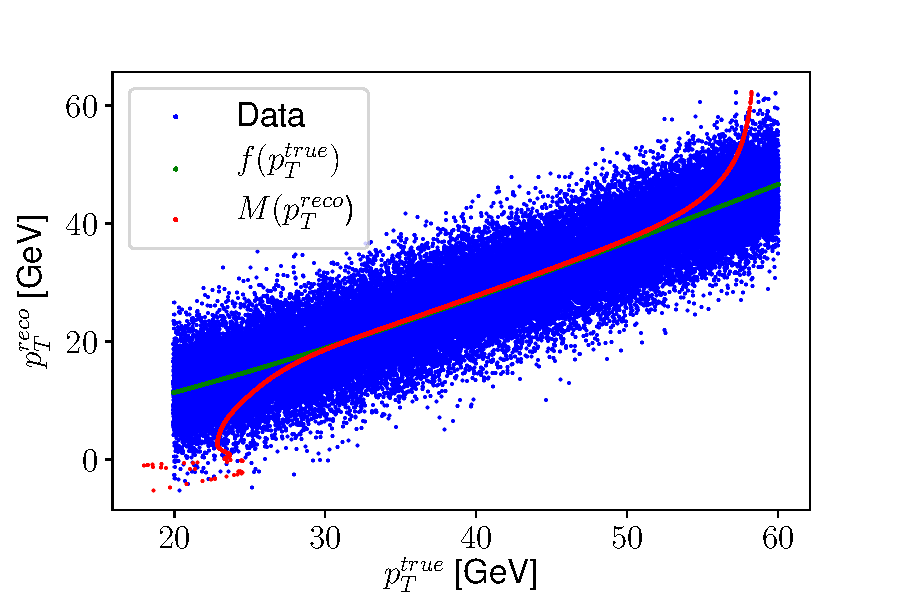
\includegraphics[width=0.45\textwidth]{{figures/nonlinearf_y_x.pdf}}}
  \subfloat[]{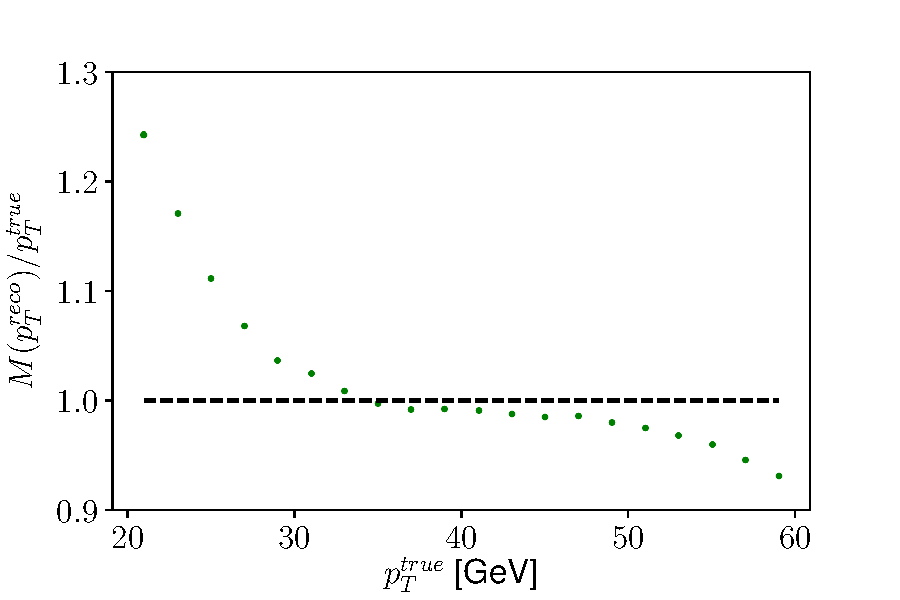
\includegraphics[width=0.45\textwidth]{{figures/nonlinearf_Myx_x.pdf}}}\\
  \subfloat[]{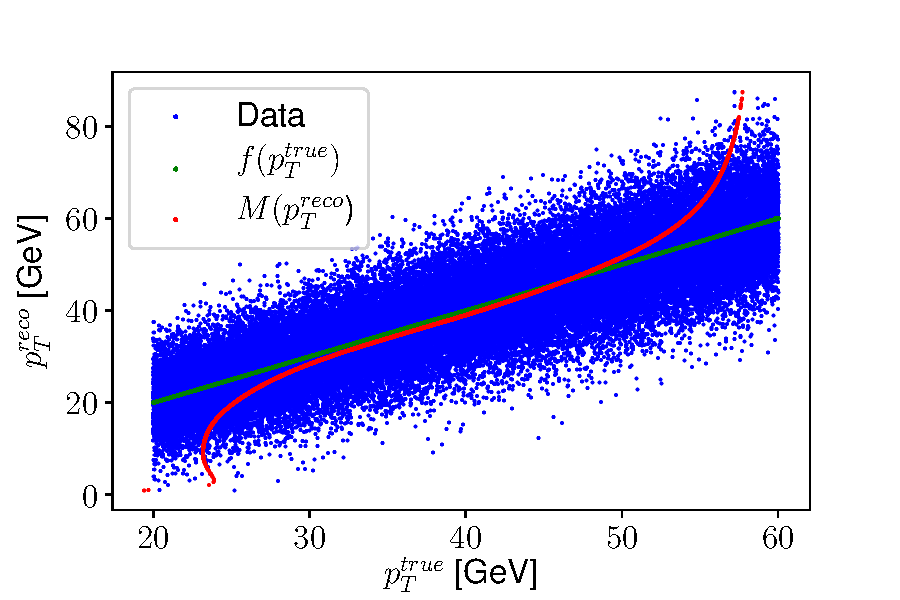
\includegraphics[width=0.45\textwidth]{{figures/nonconstantsigma_y_x.pdf}}}
  \subfloat[]{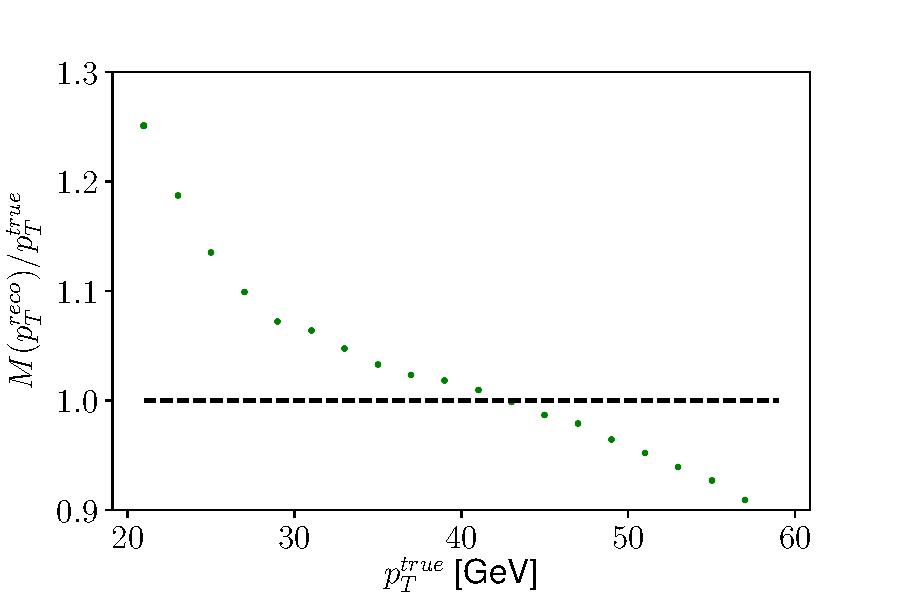
\includegraphics[width=0.45\textwidth]{{figures/nonconstantsigma_Myx_x.pdf}}}\\
  \subfloat[]{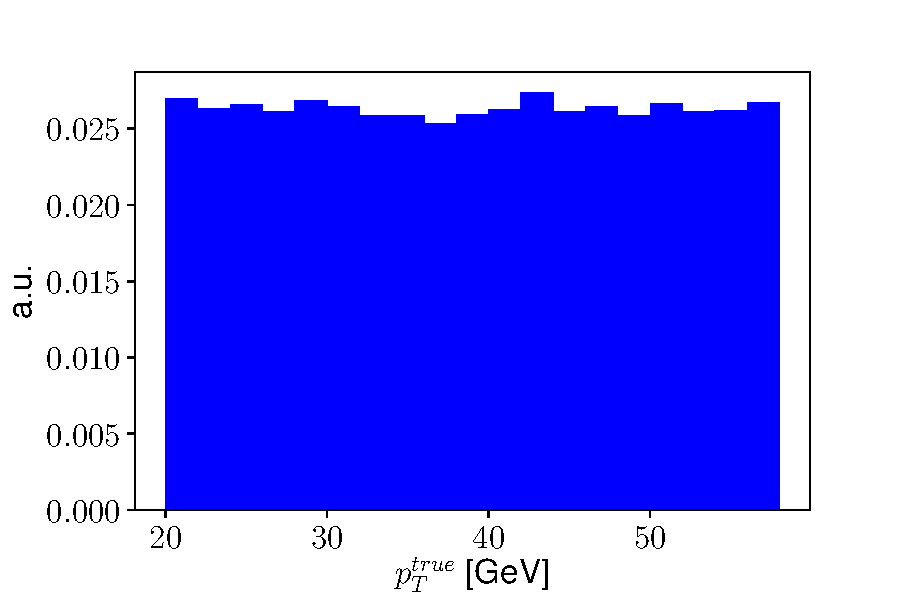
\includegraphics[width=0.45\textwidth]{{figures/uniformx.pdf}}}
  \caption{
    The effects of learning a function $M(Y)$ that predicts $X$ directly given $Y$, with a uniform underlying distribution of $X$ (e).  
    (a,b) A nonlinear $f(x)$ intended to model the ATLAS nonlinear response function, with a constant resolution.
    (c,d) A nonconstant $\sigma(Y|X=x)$ intended to model the ATLAS nonconstant resolution, with a linear $f(x)$.
    In this figure only $X$ and $Y$ correspond to the truth and reconstructed jet $\pt$, respectively, rather than the $\et$, as will be the case for the remainder of this chapter; however, the principle is exactly the same.
    }
  \label{fig:NI:learningprior}
\end{figure}

\subsection{Numerical Inversion}
\label{sec:NI:numinversion}
Instead, the ATLAS calibration uses numerical inversion. Formally, numerical inversion is the following procedure:

\begin{enumerate}
\item Compute $f(x)$, $R(x)$.  
\item Let $\tilde{R}(y) = R(f^{-1}(y))$.
\item Apply a jet-by-jet correction: $Y\mapsto Y/\tilde{R}(Y)$.
\end{enumerate}

The intuition for step 2 is that for a given value $y$ drawn from the distribution $Y|X=x$, $f^{-1}(y)$ is an estimate for $x$ and then $R(f^{-1}(y))$ is an estimate for the response at the value of $x$ that gives rise to $Y$.
Let $p(x)$ be the prior probability density function of $X=E_\text{T}$.
Since $f$ is defined conditioning on a given value of $X$, $f$ is by construction independent of $p(x)$.
Therefore, this calibration is independent of $p(x)$, since $f$ and thus $f^{-1}$ do not depend on $p(x)$.
The question of whether numerical inversion achieve closure will be discussed in detail in the following sections, but at least the definition of the calibration function is independent of the prior distribution of $X$.
This is what we mean when we say that numerical inversion is independent of the underlying spectrum.

We can see now our first result, which will be useful for the rest of this chapter:
\vspace{6mm}

\noindent{\it The correction derived from numerical inversion is $Y \mapsto Z = f^{-1}(Y)$.}

\noindent{\bf Proof.}
\begin{align}
\tilde{R}(Y) &= R(f^{-1}(Y))\nonumber\\
&= \frac{f(f^{-1}(Y))}{f^{-1}(Y)}\nonumber\\
&= \frac{Y}{f^{-1}(Y)}\nonumber\\
\rightarrow Z &= \frac{Y}{\tilde{R}(Y)}\nonumber\\
&= f^{-1}(Y) \hspace{1 cm} \Box
\end{align}
I.e., the calibration function $g$ is simply $g=f^{-1}$.

\subsection{Assumptions and Definitions}
\label{sec:NI:assumptions}

The general results presented in the following sections are based on three assumptions listed below.  These requirements should be satisfied by real detectors using calorimeters and trackers to reconstruct jets, given that the detector-level reconstruction is of sufficiently high quality.

\begin{enumerate}
\item $f^{-1}(y)$ exists for all $y$ in the support of $Y$, and $f^{-1}$ is single-valued.  These may seem like obvious statements, but are not vacuous, even for a real detector.  For example, pileup corrections can result in non-zero probability that $Y<0$, so the function $f$ must be computed for all possible values of $Y$, even if the transverse energy is negative.  At the high-luminosity LHC (HL-LHC), the level of pileup will be so high that the jet energy resolution may be effectively infinite at low transverse energies (no correlation between particle-level and detector-level jet energy).  In that case, $f^{-1}$ may not be single valued and numerical inversion cannot be strictly applied as described in Section~\ref{sec:NI:numinversion}.
\item $f(x)$ is monotonically increasing: $f'(x)>0$ for all $x$.  This condition should trivially hold for any reasonable detector: detector-level jets resulting from particle-level jets with a higher $E_\text{T}$ should on average have a higher $E_\text{T}$ than those originating from a lower $E_\text{T}$ particle-level jet.  Note that this is only true for a fixed $\eta$.  Detector technologies depend significantly on $\eta$ and therefore the $\eta$-dependence of $f$ (for a fixed $x$) need not be monotonic. We note also that Assumption 1 implies that $f'(x)\ge 0$ or $f'(x) \le 0$ for all $x$; so Assumption 2 is equivalent to the additional assumptions that $f'(x)\ne 0$ for any $x$, and that $f'(x)>0$ (as opposed to $f'(x)<0$).
\item $f$ is twice-differentiable. The first derivative of $f$ has already been assumed to exist in Assumption 2, and the second derivative will also be required to exist for some of the later results. In practice we expect $f$ to be differentiable out to any desired order.
\end{enumerate}

We note that as long as the above three assumptions hold, the theorems stated in the remainder of this chapter are valid.
In particular, this implies that $x$ could be any calibrated quantity that satisfies the above constraints.

We have separated the results in this chapter into ``Proofs'' and ``Derivations''.
The ``Proofs'' require only the three assumptions stated above, and in particular do not assume anything about the shape of the underlying distributions, e.g. that the distributions $Y|X=x$ are Gaussian or approximately Gaussian.
The ``Derivations'' are useful approximations that apply in the toy model described in Appendix~\ref{sec:NI:toy_model}; we expect them to apply in a wide variety of cases relevant to LHC jet physics.
In particular, we expect these approximations to hold in cases with properties similar to the toy model presented here - e.g., good approximation of $f$ by its truncated Taylor series about each point and approximately Gaussian underlying distributions of $Y|X=x$.
\footnote{Note that we do not require that $Y|X=x$ is exactly Gaussian, only that it is approximately Gaussian, which is true for a wide range of energies and jet reconstruction algorithms at ATLAS and CMS. In particular, there are non-negligible (but still often small) asymmetries at low and high $E_\text{T}$ at ATLAS and CMS~\cite{Aad:2011he,Chatrchyan:2011ds,Khachatryan:2016kdb}. In any case, even if $Y|X=x$ {\it is} Gaussian, $Z|X=x$ is in general {\it not} Gaussian, for non-linear response functions (Appendix~\ref{sec:NI:lemma}).}
Some of the derivations are illustrative and are included in the main body of the text; however, some derivations are moved to the Appendix (\ref{ch:NI_app}) in order to make the text more readable and highlight the main results.

Finally, in the rest of this chapter, we write $\rho_{Y|X}(y|x)$ to represent the probability distribution of $Y$ given $X=x$, and $\rho_{Z|X}(z|x)$ to be the probability distribution of $Z$ given $X=x$. A standard fact about the probability distribution from changing variables is that

\begin{align}
\rho_{Z|X}(z|x) = f'(z)\rho_{Y|X}(f(z)|x).
\label{eqn:NI:newdist}
\end{align}

To ease the notation, we will often use $\rho_Y(y)$ and $\rho_Z(z)$ interchangeably with $\rho_{Y|X}(y|x)$ and $\rho_{Z|X}(z|x)$, respectively, when it is clear (as is usually the case) that we are conditioning on some true value $x$.\footnote{In practice it is necessary to condition on a small range of $X$, e.g. $X\in[x,(1+\epsilon)x]$. If $\epsilon$ is large then there can be complications from the changing of $f(x)$ over the specified range and from the shape of the prior distribution of $X$ over the specified range.  These challenges can be solved by generating large enough Monte Carlo datasets.  We therefore assume that $\epsilon \ll 1$ and consider complications from finite $\epsilon$ beyond the scope of this Thesis.}

\section{Results}

In the subsequent sections, we will derive properties about the closure $C$ for three different definitions of the central tendency: mean (Section~\ref{sec:NI:mean}), mode (Section~\ref{sec:NI:mode}), and median (Section~\ref{sec:NI:median}).

\subsection{Mean}
\label{sec:NI:mean}

In the following section only, for brevity, we will let $f$ be $f_\text{me}$ and $C$ be $C_\text{me}$.
\subsubsection{Closure}
\label{sec:NI:meanclosuresection}

We can write the closure (Equation~\ref{eqn:NI:closure}) as

\begin{align}
C = \mathbb{E}\left[\frac{Z}{x}\middle| X=x\right] &=\frac{1}{x} \int dy \rho_{Y|X}(y|x) f^{-1}(y).
\label{eqn:NI:closuredef}
\end{align}

We find that for many functions $f$, numerical inversion does not close. This is summarized in the following result:

\vspace{5mm}

\noindent {\it Let the notion of central tendency be the mean. If $f$ is linear, then numerical inversion closes. If $f$ is not linear, then numerical inversion does not necessarily close.}

\vspace{5mm}

\noindent {\bf Proof.}
Let $f$ be linear, $f(x) = a(x+b)$. Then\footnote{We have $a>0$ from the assumption that $f'(x)>0$.} $f^{-1}(y) = \frac{y}{a}-b$. We can see that we necessarily have closure as Equation~\ref{eqn:NI:closuredef} can be written
\begin{align}
C &=\frac{1}{x} \int dy \rho_{Y|X}(y|x) \left(\frac{y}{a}-b\right)\nonumber\\
&=\frac{1}{x} \left(\frac{1}{a}\mathbb{E}\left[Y\middle| X=x\right]-b\right)\nonumber\\
&=\frac{1}{x} \left(\frac{1}{a}f(x)-b\right)\nonumber\\
&=1.
\label{eqn:NI:closure_linear_proof}
\end{align}

Now let $f$ be nonlinear, and so therefore $f^{-1}$ is also nonlinear. We note that the statement being proved is that $f$ does not necessarily close in this case; not that $f$ necessarily does not close. Thus, it is sufficient to find a counterexample that does not close in order to demonstrate this statement. Let $f(x) = \left(\frac{x}{c}\right)^{\frac{1}{3}}$ with $c\ne 0$, so that $f^{-1}(y) = cy^3$, which is a simple non-linear monotonic function. We will also need to specify some higher moments of the distribution $\rho_{Y|X}$. With the standard definitions of the variance and skew, respectively:
\begin{align}
\sigma(x)^2&\equiv
\mathbb{E}\left[\left(Y-\mathbb{E}\left[Y\right]\right)^2\middle| X=x\right]\\
\sigma(x)^3\gamma_1(x) &\equiv \mathbb{E}\left[\left(Y-\mathbb{E}\left[Y\right]\right)^3\middle| X=x\right].
\end{align}
We specify the weak conditions that $\sigma(x) >0$ (which is always true as long as $\rho_{Y|X}$ is not a delta function), and that $\gamma_1(x)=0$ (which is true if $\rho_{Y|X}$ is symmetric).  Then, the closure (Equation~\ref{eqn:NI:closuredef}) can be written
\begin{align}
C &=\frac{1}{x} \int dy \rho_{Y|X}(y|x) \left(cy^3\right)\nonumber\\
&=\frac{c}{x} \left(\mathbb{E}\left[Y^3\middle| X=x\right]\right).
\end{align}
With $\gamma_1(x)=0$, we have that
\begin{align}
\mathbb{E}\left[Y^3\middle| X=x\right] &= 3\sigma(x)^2\mathbb{E}\left[Y\middle| X=x\right] + \mathbb{E}\left[Y\middle| X=x\right]^3\nonumber\\
&=3\sigma(x)^2f(x)+f(x)^3\nonumber\\
&=3\sigma(x)^2\left(\frac{x}{c}\right)^{\frac{1}{3}}+\frac{x}{c}.
\end{align}
Then we see we do not have closure, as
\begin{align}
C &=\frac{c}{x} \left(\mathbb{E}\left[Y^3\middle| X=x\right]\right)\nonumber\\
&=\frac{c}{x} \left(3\sigma(x)^2\left(\frac{x}{c}\right)^{\frac{1}{3}}+\frac{x}{c}\right)\nonumber\\
&= 1 + 3\sigma(x)^2\left(\frac{x}{c}\right)^{-\frac{2}{3}}\nonumber\\
&>1. \hspace{1 cm}\Box
\end{align}
Although the counterexample provided here only applies to a specific choice of $f(x)$ and $\rho_{Y|X}(y|x)$, we have reason to believe that closure is not achieved for non-linear $f$ in the vast majority of cases, as can be seen in more detail in Appendix~\ref{sec:NI:mean_nonclosure}. In addition, we can Taylor expand the closure $C$ to derive an equation for the first non-closure term:
\begin{align}
C \approx 1-\frac{1}{2}\frac{f''(x)}{f'(x)^3}\frac{\sigma(x)^2}{x},
\label{eqn:NI:closureseries_text}
\end{align}
the derivation of which can be found in Appendix~\ref{sec:NI:mean_nonclosure}.

Figure~\ref{fig:NI:mean_closure} shows the inherent non-closure in numerical inversion for a toy calculation using a response function $R(x)$ that is typical for ATLAS or CMS, and the first term of the higher-order correction (Equation~\ref{eqn:NI:closureseries_text}).

\begin{figure}[]
\begin{center}
  \includegraphics[width=0.9\textwidth]{figures/{mean_closure}.pdf}
\end{center}
\caption{The closure of numerical inversion when using the mean to calibrate, using a toy model similar to conditions in ATLAS or CMS. In blue, the exact calculated closure. In red, the estimate of the closure using the first term of the higher-order correction given in Equation~\ref{eqn:NI:closureseries_text}. For details of the model, see Appendix~\ref{sec:NI:toy_model}.}
\label{fig:NI:mean_closure}
\end{figure}

\subsubsection{Calibrated Resolution}
We often care about how well we have resolved the transverse energy of the jets, which we quantify by examining the width of the calibrated resolution $Z$.

The final calibrated resolution of the reconstructed jets is defined to be the standard deviation of the $Z$ distribution, with $X=x$, which is given by
\begin{align}
\hat{\sigma}(x)^2\equiv\sigma\left(Z|X=x\right)^2 \equiv \mathbb{E}\left[Z^2\middle| X=x\right]-\mathbb{E}\left[Z\middle| X=x\right]^2,
\end{align}
and the fractional resolution is just given by $\sigma\left(\frac{Z}{x}|X=x\right)$.  The fractional resolution, to first order in the Taylor series, is given by
\begin{align}
\sigma\left(\frac{Z}{x}|X=x\right)=\frac{1}{x}\hat{\sigma}(x) \approx \frac{1}{x}\frac{\sigma(x)}{f'(x)},
\label{eqn:NI:resolutionseries_text}
\end{align}
the derivation of which can be found in Appendix~\ref{sec:NI:calibrated_resolution_calculation}.  Note that $f'(x)$ is \emph{not} the response $R(x)=\frac{f(x)}{x}$. In particular, $f'(x)=R(x)+R'(x)x$, so $f'(x)\ne R(x)$ unless $R'(x)=0$, or equivalently $f(x)= kx$ for some constant $k$ (which is not the case at ATLAS nor at CMS). Figure~\ref{fig:NI:mean_resolution} verifies Equation~\ref{eqn:NI:resolutionseries_text} and compares it to the method of dividing the width of the distribution by $R$, which is a standard diagnostic technique when a full calibration is not applied.

\begin{figure}
\begin{center}
  \includegraphics[width=0.9\textwidth]{figures/{mean_resolution}.pdf}
\end{center}
\caption{The resolution of the $E_\text{T}$ distribution following numerical inversion when using the mean to calibrate, using a toy model similar to conditions in ATLAS or CMS. In blue, the exact calculated resolution. In red, the estimate of the closure using the first term of the higher-order correction in Equation~\ref{eqn:NI:resolutionseries_text}. In green, the uncalibrated resolution. In orange, the resolution when dividing by the response $R(x)$. For details of the model, see Appendix~\ref{sec:NI:toy_model}.}
\label{fig:NI:mean_resolution}
\end{figure}

\subsection{Mode}
\label{sec:NI:mode}
In the following section only, for brevity, we will let $f$ be $f_\text{mo}$ and $C$ be $C_\text{mo}$.  The distribution $\rho_{Y|X}(y|x)$ is usually unimodal and Gaussian fits to the ``core'' of this distribution are essentially picking out the mode of the distribution.  Therefore, the results of this section are a good approximation to what is often used in practice. We note that in the case that the underlying distribution is multimodal, it is not clear how to unambiguously define the mode of the distribution, and so the results of this section cannot be applied naively.

\subsubsection{Closure}
\label{sec:NI:modeclosuresection}
Assuming that the probability distribution function is unimodal, the mode is the point at which the first derivative of the function is 0:
\begin{align}
f(x) = y^* \text{ s.t. } \rho'_Y(y^*) = 0.
\label{eqn:NI:modedef}
\end{align}
Then we can write the closure condition (Equation~\ref{eqn:NI:closure}) as
\begin{align}
\text{mode}\left[\frac{Z}{x}\middle| X=x\right] = 1\nonumber\\
\rightarrow \text{mode}\left[Z\middle| X=x\right] = x\nonumber\\
\rightarrow \rho'_Z(x) = 0.
\label{eqn:NI:modeclosuredef}
\end{align}

\noindent Using this definition, we can prove a result similar (but stronger) to the closure condition for the mean in the previous section:

\vspace{5mm}

\noindent  {\it Let the notion of central tendency be the mode. Numerical inversion closes if and only if $f$ is linear.}

\vspace{5mm}

\noindent  {\bf Proof.} We have from Equation~\ref{eqn:NI:newdist} that
\begin{align}
\rho_Z(z) = f'(z)\rho_Y(f(z)).
\end{align}
Therefore,
\begin{align}
\rho'_Z(z) = f''(z)\rho_Y(f(z))+f'(z)^2\rho'_Y(f(z)),
\end{align}
and
\begin{align}
\rho'_Z(x) &= f''(x)\rho_Y(f(x))+f'(x)^2\rho'_Y(f(x))\nonumber\\
&=f''(x)\rho_Y(y^*)+f'(x)^2\rho'_Y(y^*)\nonumber\\
&=f''(x)\rho_Y(y^*),
\end{align}
where $\rho_Y(y^*)>0$ since $y^*$ is the mode of the distribution $\rho_Y$. Then we see that if $f''(x)=0$, then $\rho'_Z(x)=0$ and closure is achieved.  In contrast, if $f''(x)\ne 0$, then $\rho'_Z(x)\ne 0$ and closure is not achieved. $\hspace{0.5 cm}\Box$

\vspace{5mm}

\noindent The closure when using the mode to calibrate, to first order in the Taylor series, is given by
\begin{align}
C \approx 1+\frac{f''(x)}{f'(x)^3}\frac{\tilde{\sigma}(x)^2}{x},
\label{eqn:NI:closure_mode_text}
\end{align}
where $\tilde{\sigma}(x)$ is the width of a Gaussian fitted to just the area near the peak of the function $\rho_{Y|X}(y|x)$ (defined precisely in the next section). The derivation of Equation~\ref{eqn:NI:closure_mode_text} can be found in Appendix~\ref{sec:NI:calibrated_mode_calculation}.

Figure~\ref{fig:NI:mode_closure} shows the inherent non-closure in numerical inversion for a toy calculation using a response function $R(x)$ that is typical for ATLAS or CMS, and the first term of the higher-order correction given in Equation~\ref{eqn:NI:closureseries_text}, when using the mode for calibration.

\begin{figure}[]
\begin{center}
  \includegraphics[width=0.9\textwidth]{figures/{mode_closure}.pdf}
\end{center}
\caption{The closure of numerical inversion when using the mode to calibrate, using a toy model similar to conditions in ATLAS or CMS. In blue, the exact calculated closure. In red, the estimate of the closure using the first term of the higher-order correction given in Equation~\ref{eqn:NI:closure_mode_text}. For details of the model, see Appendix~\ref{sec:NI:toy_model}.}
\label{fig:NI:mode_closure}
\end{figure}

\subsubsection{Resolution}
Let $z^*(x)$ be the mode of the distribution $Z|X=x$, which is not necessarily equal to $x$ given the above result. It is often the case at ATLAS and CMS that a Gaussian is fit to the distributions $\rho_{Y|X}(y|x)$ and $\rho_{Z|X}(z|x)$ only in the vicinity of the modes $f(x)$ and $z^*(x)$, respectively, since it is assumed that the distributions have a Gaussian core but non-Gaussian tails. The width of the Gaussian core found in this fit is then used as a measure of the resolution of the distribution.  We thus define a ``trimmed resolution'' for a distribution $P$ with probability distribution function $\rho_P(p)$ about its mode $m$, which is valid if $P\sim\mathcal{N}(m,\tilde{\sigma})$ for $p$ near $m$:
\begin{align}
\label{eq:tildesigma}
\tilde{\sigma}(P)^2 \equiv -\frac{\rho_P(m)}{\rho_P''(m)}.
\end{align}

\noindent The definition in Equation~\ref{eq:tildesigma} is chosen because it reduces to the usual variance for a Gaussian distribution.  For the distributions $\rho_{Y|X}(y|x)$ and $\rho_{Z|X}(z|x)$, we thus have the trimmed resolutions
\begin{align}
\tilde{\sigma}(x)^2\equiv\tilde{\sigma}\left(Y|X=x\right)^2 = -\frac{\rho_Y(f(x))}{\rho_Y''(f(x))} \\
\hat{\tilde{\sigma}}(x)^2\equiv\tilde{\sigma}\left(Z|X=x\right)^2 = -\frac{\rho_Z(z^*(x))}{\rho_Z''(z^*(x))}.
\label{mode_resolution_def}
\end{align}

\noindent The calibrated fractional trimmed resolution $\tilde{\sigma}\left(\frac{Z}{x}|X=x\right)$, to first order in the Taylor series, is given by
\begin{align}
\tilde{\sigma}\left(\frac{Z}{x}|X=x\right) = \frac{1}{x}\hat{\tilde{\sigma}}(x) \approx \frac{1}{x}\frac{\tilde{\sigma}(x)}{f'(x)},
\label{eqn:NI:resolutionmode_text}
\end{align}
the derivation of which can be found in Appendix~\ref{sec:NI:mode_resolution_calculation}.

\subsection{Median}
\label{sec:NI:median}
In the previous sections we have examined using the mean or the mode to define $f$ and $C$, and found that both results do not lead to closure in general. We propose a new definition, using the median of the reconstructed jet $E_\text{T}$ distributions:
\begin{align}
f_\text{med}(x)&=\text{median}[Y|X=x]\\
R_\text{med}(x) &= \text{median}\left[\frac{Y}{x}\middle| X=x\right] = \frac{f_\text{med}(x)}{x}. 
\end{align}
And define $C_\text{med}$ analogously.  In the following section only, for brevity, we will let $f$ be $f_\text{med}$ and $C$ be $C_\text{med}$.
\subsubsection{Closure}
\label{sec:NI:medianclosuresection}
The median of the distribution is the point at which 50\% of the distribution is above and 50\% is below:
\begin{align}
f(x) = y^* \text{ s.t. } \int_{-\infty}^{y^*} \rho_Y(y) dy = 0.5.
\end{align}
Then the closure condition (Equation~\ref{eqn:NI:closure}) can be written
\begin{align}
\text{median}\left[\frac{Z}{x}\middle| X=x\right] = 1\nonumber\\
\rightarrow \text{median}\left[Z\middle| X=x\right] = x\nonumber\\
\rightarrow \int_{-\infty}^{x} \rho_Z(z) dz = 0.5.
\label{eqn:NI:medianclosuredef}
\end{align}
We can see then the following result under this definition of central tendency:

\vspace{5mm}

\noindent {\it Let the notion of central tendency be the median. Then numerical inversion always closes.}

\vspace{5mm}

\noindent {\bf Proof.} We have from Equation~\ref{eqn:NI:newdist} that
\begin{align}
\rho_Z(z) = f'(z)\rho_Y(f(z)).
\end{align}
So the closure condition in Equation~\ref{eqn:NI:medianclosuredef} becomes
\begin{align}
0.5 &= \int_{-\infty}^{x} \rho_Z(z) dz\nonumber\\
&=\int_{-\infty}^{x} f'(z)\rho_Y(f(z)) dz.
\end{align}
Then with $u = f(z), du = f'(z) dz$ we have
\begin{align}
0.5 &= \int_{-\infty}^{f(x)} \rho_Y(u) du\nonumber\\
&=\int_{-\infty}^{y^*} \rho_Y(u) du\nonumber\\
&=0.5. \hspace{1 cm} \Box
\end{align}

\subsubsection{Resolution}
A natural definition of resolution when using the median to calibrate jets is the 68\% interquantile range, defined as follows for a distribution $P$ with probability density function $\rho_P(p)$:

\noindent With $I_P^-$ and $I_P^+$ defined by
\begin{align}
\int_{-\infty}^{I_P^-}\rho_P(p)dp \equiv \Phi(-1),\\
\int_{-\infty}^{I_P^+}\rho_P(p)dp \equiv \Phi(+1);
\end{align}
the 68\% interquantile range is defined as
\begin{align}
\sigma_\text{IQR}(P) \equiv \frac{1}{2}\left(I_P^+-I_P^-\right).
\end{align}
Where $\Phi(x)=\frac{1}{2}\text{erfc}\left(\frac{-x}{\sqrt{2}}\right)$ is the cumulative distribution function of the normal distribution. The definition is designed so that if $P\sim\mathcal{N}(\mu,\sigma)$ then $\sigma_\text{IQR}(P)=\sigma$. The quantity $\sigma_\text{IQR}$ is called the ``68\% interquantile range'' because $\Phi(+1)-\Phi(-1) \approx 0.68$.  For the distributions $Y|X=x$ and $Z|X=x$, define:

\begin{align}
\sigma_\text{IQR}(x) = \sigma_\text{IQR}(Y|X=x)\\
\hat{\sigma}_\text{IQR}(x) = \sigma_\text{IQR}(Z|X=x).
\end{align}

\noindent Then we can see the following result for the calibrated resolution $\sigma_\text{IQR}(\frac{Z}{x}|X=x)$:

\vspace{5mm}

\noindent {\it The 68\% IQR of the calibrated response distribution is given by $\sigma_\text{IQR}(\frac{Z}{x}|X=x) = \frac{1}{2x}\left(f^{-1}(I_Y^+)-f^{-1}(I_Y^-)\right)$.}

\vspace{5mm}

\noindent {\bf Proof.}
We have
\begin{align}
\int_{-\infty}^{I_Z^-}\rho_Z(z)dz = \Phi(-1)\\
\int_{-\infty}^{I_Z^+}\rho_Z(z)dz = \Phi(+1).
\end{align}
From Equation~\ref{eqn:NI:newdist},
\begin{align}
\rho_Z(z) = f'(z)\rho_Y(f(z)),
\end{align}
so that
\begin{align}
\Phi(-1) &= \int_{-\infty}^{I_Z^-}f'(z)\rho_Y(f(z))dz\nonumber\\
&=\int_{-\infty}^{f(I_Z^-)}\rho_Y(u)du\nonumber\\
\rightarrow f(I_Z^-) &= I_Y^-\\
\Phi(+1) &= \int_{-\infty}^{I_Z^+}f'(z)\rho_Y(f(z))dz\nonumber\\
&=\int_{-\infty}^{f(I_Z^+)}\rho_Y(u)du\nonumber\\
\rightarrow f(I_Z^+) &= I_Y^+.
\end{align}
Therefore,
\begin{align}
\sigma_\text{IQR}(Z|X=x) &= \frac{1}{2}\left(I_Z^+-I_Z^-\right)\nonumber\\
&=\frac{1}{2}\left(f^{-1}(I_Y^+)-f^{-1}(I_Y^-)\right),
\end{align}
and
\begin{align}
\sigma_\text{IQR}\left(\frac{Z}{x}|X=x\right)=\frac{1}{2x}\left(f^{-1}(I_Y^+)-f^{-1}(I_Y^-)\right).\hspace{1 cm}\Box
\label{eqn:NI:resolutionmedian_text}
\end{align}
%-------------------------------------------------------------------------------
\newpage
\section{Discussion}
\label{sec:NI:discussion}

After a quick summary in Section~\ref{sec:NI:summary} of the results presented so far, Section~\ref{sec:NI:recommendations} discusses the benefits and drawbacks of various methods of calibration, and Sections~\ref{sec:NI:iterated_text} and~\ref{sec:NI:corrected_numerical_inversion_text} describe extensions of numerical inversion that may help to improve closure.

\subsection{Summary of Results}
\label{sec:NI:summary}
In Section~\ref{sec:NI:introclosure} we defined the concept of closure in the process of calibrating the $E_\text{T}$ of jets.  We found in Sections~\ref{sec:NI:meanclosuresection} and~\ref{sec:NI:modeclosuresection} that when using the mean or mode, respectively, of the distribution $Y|X=x$ to calibrate, closure is not necessarily achieved; with the response functions found at ATLAS or CMS, it is expected that numerical inversion will not close. We also provided estimates for the non-closure for the mean (Equation~\ref{eqn:NI:closureseries_text}) and for the mode (Equation~\ref{eqn:NI:closure_mode_text}). In those estimates we find that as the underlying resolution $\sigma(x)$ or $\tilde{\sigma}(x)$ of the uncalibrated jet distribution $Y|X=x$ increases, the non-closure gets worse. This indicates that the non-closure issues raised in this chapter will become more important as the LHC moves to conditions with higher pileup in the future.

\vspace{2mm}

A new calibration scheme based on the median of $Y|X=x$ is proposed in Section~\ref{sec:NI:medianclosuresection}.  With this method of calibration, closure is always achieved.

\vspace{2mm}

Each section also explored various definitions of the resolution of the fractional calibrated jet distribution $\frac{Z}{x}|X=x$, where the most natural definition depends on the manner in which calibration has been performed (i.e., whether using the mean, mode, or median to calibrate). We provided useful estimates for the standard deviation (Equation~\ref{eqn:NI:resolutionseries_text}), the trimmed Gaussian width (Equation~\ref{eqn:NI:resolutionmode_text}), and an exact formula for the 68\% IQR (Equation~\ref{eqn:NI:resolutionmedian_text}). These expressions can be used to quickly estimate the final resolution of a jet algorithm without having to actually apply the calibration jet-by-jet.

\subsection{Recommendation for Method of Calibration}
\label{sec:NI:recommendations}
As mentioned in the summary above, we have that for a non-linear response function closure is not necessarily achieved when using the mode or mean to calibrate, and closure is necessarily achieved when using the median. While this indicates that the median is a useful metric to use if closure is the main objective, we accept that there might be reasons to use the mode instead (for example, if the tails of $\rho_{Y|X}(y|X=x)$ are cut off, then the mode should stay constant while the median and mean will change). Thus we leave it to the reader to decide which method of calibration is most appropriate to use for their specific purposes. To that end, we also have discussion below about methods to improve the closure when the mode is being used to calibrate.

\subsection{Iterated Numerical Inversion}
\label{sec:NI:iterated_text}
A natural question is whether it is useful for the purposes of achieving closure to implement numerical inversion again on the calibrated jet collection, if closure has not been achieved the first time. We define the \emph{iterated numerical inversion} process as follows:

\vspace{5mm}

\noindent With $C(x)$ defined as in Equation~\ref{eqn:NI:closure}, let
\begin{align}
R_{\text{new}}(x) &\equiv C(x)\\
f_{\text{new}}(x) &\equiv C(x)x.
\end{align}
Then, apply numerical inversion on the calibrated distribution $Z$:
\begin{align}
Z\mapsto Z_\text{new} = f_{\text{new}}^{-1}(Z).
\end{align}
We then ask if the closure of this new distribution, $C_\text{new}(x)$ (defined analogously as in Equation~\ref{eqn:NI:closure}), is closer to 1 than $C(x)$.  In general, this is a difficult question to answer, but we have derived analytic approximations when the mode is used to derive the calibration (Appendix~\ref{sec:NI:iterated}).  Iterating numerical inversion does \emph{not} always help:

\begin{align}
\frac{|C_\text{new}(x)-1|}{|C(x)-1|} &\approx \frac{12f''(x)^2\tilde{\sigma}(x)^2}{f'(x)^4}\label{eqn:NI:iterated_closure_ratio}.
\end{align}
If the ratio in Equation~\ref{eqn:NI:iterated_closure_ratio} is greater than 1, then the closure gets worse after a second iteration of numerical inversion.  In particular, as $\tilde{\sigma}(x)$ gets larger, the iterated closure gets worse relative to the original closure. So we expect at higher levels of pileup that iterating numerical inversion will not be useful. In Figure~\ref{fig:NI:mode_closure_bigs} we can see that iterating numerical inversion does make the closure worse than the original closure, in a model simulating higher pileup conditions.  The next section provides another scheme to correct for the residual non-closure that does not require iterating the process of numerical inversion.

\subsection{Corrected Numerical Inversion}
\label{sec:NI:corrected_numerical_inversion_text}
As noted above, when using the mean or mode of the distribution $Y|X=x$ to calibrate, closure is not achieved in general. With the closed-form estimates of the non-closure provided in the text, one might think to simply ``subtract off'' the non-closure. However the non-closure estimates provided are in terms of the truth $E_\text{T}$ value $x$.  Since $x$ is not available in data, a sensible proxy is to use numerical inversion as an estimate for $x$.  This is actually equivalent to iterated numerical inversion, which as shown in the previous section does not always help.

Another possibility is to use a different original response function to perform the calibration.  Suppose that instead of using $f(x)=R(x)x$, there was a new function $g(x)\ne f(x)$ such that if the calibration is performed with this new function, $Y\mapsto Z_\text{corr}=g^{-1}(Y)$, the new calibrated distribution $Z_\text{corr}|X=x$ does achieve closure or gets closer to achieving closure than when calibrating using $f$.

We define the \emph{corrected numerical inversion} process as follows:
\begin{enumerate}
\item Calculate $f(x)=f_\text{mo}(x)=\text{mode}[Y|X=x]$.
\item Let $g(x) = g(x;f(x))$ be a calibration function depending on the fitted function $f(x)$.
\item Apply the calibration $Y\mapsto Z_\text{corr}=g^{-1}(Y)$ jet-by-jet.
\end{enumerate}
We then can examine the closure
\begin{align}
C_\text{corr}(x) = \text{mode}\left[\frac{Z_\text{corr}}{x}\Big|X=x\right].
\end{align}
And say we have achieved closure if
\begin{align}
C_\text{corr}(x) \equiv 1.
\end{align}
We examine the case of using the mode to measure closure, again because in practice that is what is often used when there are significant non-Gaussian tails. 

One way to specify $g$ is by explicitly requiring closure. In Appendix~\ref{sec:NI:corrected_numerical_inversion_calculation} it is shown that in the case that closure is achieved exactly, $g$ necessarily satisfies the differential equation\footnote{As noted in the derivation, this equation also assumes the following: that the underlying distribution $Y|X=x$ is approximately Gaussian in the vicinity of its mode $f(x)$; and that the correction is small, with $|g(x)-f(x)|\ll \tilde{\sigma}(x)$.}
\begin{align}
0=g''(x)-g'(x)^2\frac{g(x)-f(x)}{\tilde{\sigma}(x)^2}.
\label{eqn:NI:diffeq}
\end{align}
In principle Equation~\ref{eqn:NI:diffeq} can be solved numerically given numerical fitted values $f(x)$ and $\tilde{\sigma}(x)$, though in practice such a method may prove intractable.

Another way to specify $g$ is to use external parameters
\begin{align}
g(x) = g(x;f(x);a_1,...,a_n).
\end{align}
Then the parameters $a_1,...,a_n$ can be chosen such that the closure is as close to 1 as possible. This is the method used to find the corrected calibration curve in Figure~\ref{fig:NI:mode_closure_bigs}, and explained in more detail in Appendix~\ref{sec:NI:corrected_numerical_inversion_parameterization}. The absolute non-closure $|C-1|$ is significantly smaller than the original non-closure, even in a model simulating very high pileup conditions.

\begin{figure}[]
\begin{center}
  \includegraphics[width=0.9\textwidth]{figures/{mode_closure_bigs}.pdf}
\end{center}
\caption{The top plot shows the closure of numerical inversion when using the mode to calibrate, using a toy model similar to conditions in ATLAS or CMS but increasing $\sigma(x)$ by a factor of 1.4 in order to simulate higher pileup conditions. In blue, the original closure as defined in Equation~\ref{eqn:NI:closure}. In green, the closure after iterating numerical inversion once as in Section~\ref{sec:NI:iterated_text}. In orange, the closure after using the parameterized corrected numerical inversion technique as in Section~\ref{sec:NI:corrected_numerical_inversion_text}. For details of the model, see Appendix~\ref{sec:NI:toy_model}. The bottom plot shows the absolute non-closure $|C-1|$. In particular, at low $E_\text{T}$, iterating numerical inversion does worse, while corrected numerical inversion does better than the original calibration.}
\label{fig:NI:mode_closure_bigs}
\end{figure}

%-------------------------------------------------------------------------------









%-------------------------------------------------------------------------------
\section{Conclusions}
\label{sec:NI:conclusion}
%-------------------------------------------------------------------------------

Jets are ubiquitous at the LHC and are used extensively in the two main searches presented in this Thesis (Chapter~\ref{ch:HBSM} and Chapter~\ref{ch:CWoLa}).
The calibration of the energy and mass of jets is necessary for their practical use in these analyses or any other, and understanding and improving this calibration can improve the sensitivity to new physics.
The standard technique used for jet calibration at ATLAS and at CMS is numerical inversion.
This chapter serves to formally define numerical inversion and derive many of its properties.

This study has resulted in a few novel discoveries and clarifications about this standard technique.

It is firmly established that numerical inversion does achieve its key property, which is that it is independent of the underlying distribution used to derive the calibration.

However, numerical inversion is established to be inherently biased: when using the mean or mode of the reconstructed kinematic distributions to calibrate, the calibrated response function does not close, if the uncalibrated response function is nonlinear.
The size of this nonclosure is approximated for the first time and is shown to get worse as the resolution of jets gets worse, in particular as is expected as the LHC moves to higher instantaneous luminosity and pile-up conditions in the future.
When using the median as the notion of central tendency, the method is guaranteed to close.
However, there are good reasons to use the mode instead of the median, and we do not recommend one method over the other because of these respective drawbacks.

An approximation for the the calibrated jet resolution is provided which can be used to estimate the resolution before actually doing the calibration.
Previously, a common approach to do this estimation was to divide the uncalibrated resolution by the uncalibrated response, but this approach is shown to be inaccurate.
Instead, our approximation uses the derivative of the uncalibrated response, and is shown to be more accurate.

Given the inherent nonclosure present in numerical inversion, the question of whether numerical inversion can be improved is answered in a couple different ways. 
First, simply iterating numerical inversion is shown for the first time to not always help.
Second, an extension is proposed in which a modified calibration function can be constructed to achieve a better closure than the standard technique.

In addition to the corrections and extensions proposed, the deep understanding generally of numerical inversion provided for the creation of the technique described in Chapter~\ref{ch:Calib}.
The realization that numerical inversion was defined by a single function (Section~\ref{sec:NI:numinversion}), and that this function could be modified to achieve better closure, led directly to the idea that this function could be approximated with a neural network, which could simultaneously and automatically take into account multiple auxiliary variables.

While this Thesis focuses on the use of jets at the LHC, numerical inversion is in fact a generic detector calibration method that can be applied as long as there is a reliable method for matching the value of an observable before and after passing through the detector (either via simulation or high-fidelity calibration data).
The results presented here therefore can be applied to objects other than jets at the LHC, or indeed even beyond the realm of high energy physics.

\clearpage
\newpage
